% TEXINPUTS=templates/LaTeX2e//: pdflatex paper1_iberamia_timeformer.tex
% TEXINPUTS=templates/LaTeX2e//: bibtex paper1_iberamia_timeformer
% TEXINPUTS=templates/LaTeX2e//: pdflatex paper1_iberamia_timeformer.tex
% TEXINPUTS=templates/LaTeX2e//: pdflatex paper1_iberamia_timeformer.tex
%
% This file is intentionally a planning skeleton, not a full manuscript draft.
\documentclass[runningheads]{llncs}

\usepackage[T1]{fontenc}
\usepackage{graphicx}
\usepackage{amsmath}
\usepackage{amssymb}
\usepackage{booktabs}

\begin{document}

% Candidate titles (most evaluation-centric is active):
% [A] Temporal Traceability in Transformer Representations: A Controlled Diagnostic Evaluation
% [B] Geometric Temporal Traceability: Controlled Diagnostics for Transformer Conditioning Architectures
% [C] Amnesia by Design: Diagnosing Temporal Traceability in Transformer Representations
\title{Amnesia by Design: Diagnosing Temporal Traceability in Transformer Representations}
\titlerunning{Amnesia by Design: Temporal Traceability in Transformer Representations}

\author{Anonymous Author}
\authorrunning{Anonymous}

\institute{Institution withheld for review}

\maketitle

\begin{abstract}
Words do not preserve fixed meanings across time. \texttt{gay@1920} and
\texttt{gay@1980} are different semantic objects, yet transformers represent
both in a shared geometric space. Masked language modeling rewards correct
token prediction rather than geometric consistency across time, so
\emph{temporal traceability} (whether a token occupies different representational
neighborhoods at different periods) is not directly optimized.

Our central contribution is a controlled diagnostic suite with planted
trajectories (stable, drifting, bifurcating) and a diagnostic battery targeting
neighborhood geometry; using it we evaluate temporal conditioning architectures
against non-temporal (Standard) and global-signal (Additive) baselines.
Conditioning of any form substantially increases neighborhood drift for drifting
subjects relative to Standard; Additive and joint token-time conditioning
(Token-Time) produce equivalent aggregate drift, with a reproducible advantage
for Token-Time appearing only when local markers are removed (ambiguous split,
probe accuracy 0.595 vs.\ 0.579). The Memory-Augmented extension exposes
mean-prototype aggregation as a second failure mode: when a word develops
coexisting senses, a mean prototype collapses both into a centroid that
represents neither.

The results matter for applications requiring word meaning at a specific
period. They suggest that temporal traceability requires training objectives
aligned with trajectory geometry.

\keywords{Temporal semantics \and Semantic change \and Transformer models \and Traceability \and Diagnostic evaluation}
\end{abstract}

\section{Introduction}
% Target length: 1.0--1.25 pages.
Words do not preserve fixed meanings across time. In 1900, \emph{broadcast}
referred to scattering seeds across a field; today it describes a social media
post reaching millions of users. Whether the shift of \emph{gay} from
\emph{cheerful} to its contemporary sense involved movement toward or away
from stigmatized terms~\cite{hamilton2016diachronic} is an empirical question
that requires \texttt{gay@1920} and \texttt{gay@1980} as directly comparable
objects in a shared geometric space.

Contextualized embeddings disambiguate senses through local sentential context,
not period: \emph{virus} is represented differently near \emph{malware} than
near \emph{infection}, regardless of the year. The limitation appears when one
wants \texttt{token@time} as a directly inspectable object; diachronic analysis
asks where a meaning moved, not which sense local context happens to
select.

Masked language modeling masks a token and asks the model to reconstruct it
from its neighbors. To do this well, the model learns local context; it has no
direct incentive to place the same token in period-appropriate regions of the
representation space. Temporal traceability means that \texttt{virus@1900} and
\texttt{virus@2020} occupy different neighborhoods. It requires a training
signal aligned with geometric consistency across time, which the MLM objective
does not provide.

Testing this limitation requires a controlled environment where the correct answer
is known. Natural-language corpora entangle semantic change with frequency,
genre, and subcorpus shifts, making it hard to attribute a representational
effect to architecture rather than data.

Against this diagnostic suite we evaluate temporal conditioning architectures:
a non-temporal baseline (Standard), a global-signal baseline (Additive), joint
token-time conditioning (Token-Time), and a memory-augmented extension. The
central empirical question is whether conditioning of any form improves
geometric traceability over the non-temporal baseline, and what the form of
conditioning contributes. Adjudication between conditioning forms across noisier
regimes and natural corpora is left for future work.

The paper makes four contributions. (1)~We establish temporal traceability as
a geometric property distinct from period-label recoverability, and motivate
why the MLM objective does not directly optimize it. (2)~We introduce a
controlled diagnostic suite with planted trajectories (stable, drifting,
bifurcating) and a diagnostic battery separating neighborhood geometry from
label recoverability. (3)~Using this suite we show that conditioning of any
form substantially improves geometric drift over the non-temporal baseline, and
that the conditioning form is not separable on aggregate drift in this regime
(preliminary separation appears only when local markers are removed). (4)~We
identify mean-prototype aggregation as a failure mode for bifurcating subjects.


\section{Related Work}
% Target length: under 1 page.
Lexical semantic change detection (LSCD) is the dominant computational framing
for meaning shift. Diachronic word embeddings~\cite{hamilton2016diachronic}
learn one distributional space per time slice, align independently trained
models, and measure movement in neighborhood structure. We share the intuition
that semantic change is geometric, but not the architecture: LSCD yields a
scalar comparison between spaces rather than a jointly parameterized
\texttt{token@time} representation. Standard benchmarks formalize this
task~\cite{schlechtweg2020semeval,tahmasebi2021survey}, while also inheriting
natural-corpus confounds such as frequency and genre drift; shared tasks for
Spanish show that manual annotation is required even for modern
corpora~\cite{zamora2022lscdiscovery}. Our controlled diagnostic suite plants trajectories so that traceability is
attributed to model design, not corpus composition.

Temporal neural language models avoid separate spaces by conditioning one model
on time. Prior work uses timestamps for knowledge-intensive QA, masked language
modeling, or period-stratified downstream
evaluation~\cite{dhingra2022timeaware,rosin2022timemasking,loureiro2022timelms}. These results show that temporal conditioning can improve period-appropriate
prediction but do not test whether the same token occupies different
representational neighborhoods at different periods, which is the geometric
question this work addresses.

Linear probes provide another partial view. A period probe measures whether time
is recoverable from a hidden state, not whether a token has moved to a different
semantic neighborhood. We therefore report probe accuracy as auxiliary evidence
and treat neighborhood movement as the primary criterion for traceability.

Finally, semantic change may involve bifurcation rather than monotonic drift.
Giulianelli et al.\ show that words can develop coexisting
senses~\cite{giulianelli2020analysing}; mean-pooled representations then collapse
both senses into a centroid that represents neither. Our stable, drifting, and
bifurcating trajectories test this distinction directly, and the memory
extension exposes where mean-pooled prototypes fail.

\section{Controlled Diagnostic Suite}
% Target length: 1.0 page.
The diagnostic suite gives each subject a known temporal trajectory, making it
possible to ask directly whether a model's representation of a subject at \(t0\)
has moved toward the expected neighborhood by \(t9\). This distinguishes it from
natural-language LSCD benchmarks, where ground truth is often annotated or
inferred post-hoc and corpus confounds are hard to separate from genuine semantic
change.

The corpus uses a subject--verb--object (SVO) grammar: every sentence consists
of one subject, one verb, and one object. Two semantic neighborhoods, $N_1$ and $N_2$,
partition the vocabulary of 8 verbs and 8 objects: $N_1$ uses
\(\{V1,\ldots,V4\}\) and \(\{O1,\ldots,O4\}\); $N_2$ uses
\(\{V5,\ldots,V8\}\) and \(\{O5,\ldots,O8\}\). A sentence generated from
$N_1$ therefore looks like \texttt{S5 V2 O3}, while one from $N_2$
looks like \texttt{S5 V6 O8}; the subject token is the same in both cases, but
its co-occurring words differ. Intuitively, the intended meaning of subject
\(s\) at period \(t\) is how often it appears in $N_1$ sentences; formally,
\(P(N_1 \mid s, t)\) is the probability that a sentence is drawn from $N_1$.
The vocabulary contains 30 subjects; each subject's trajectory is determined by
how \(P(N_1 \mid s, t)\) evolves across the 10 periods \(t0\) through \(t9\).

\begin{figure}[t]
\centering
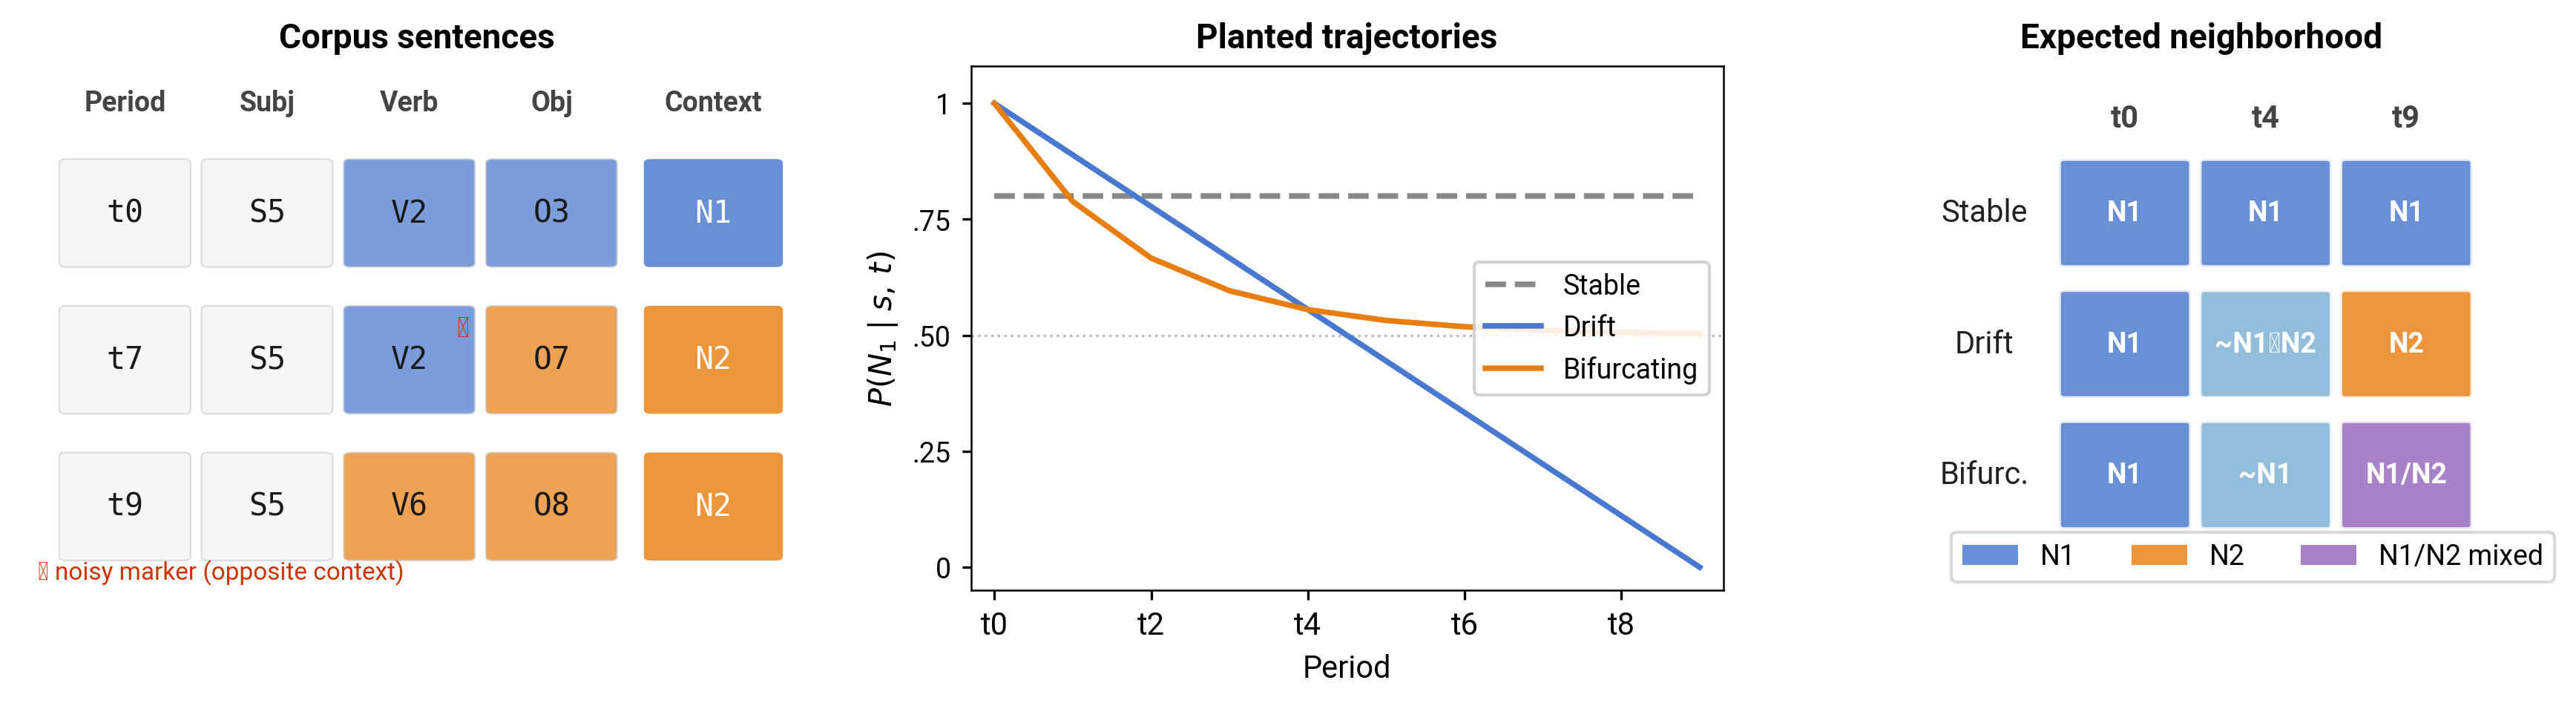
\includegraphics[width=\textwidth]{outputs/figures/figure1_benchmark_design.png}
\caption{Controlled diagnostic suite overview. \emph{Left}: SVO sentences for a drifting
subject across three periods; an $N_1$ verb appearing in an $N_2$ sentence
at \(t7\) (marked \({\ast}\)) illustrates the deliberate noise in local markers.
\emph{Center}: planted \(P(N_1 \mid s, t)\) trajectories for Stable (flat),
Drift (monotonic), and Bifurcating (levelling at 0.5) subjects across
\(t0\)--\(t9\). \emph{Right}: expected nearest-neighbor behavior for a traceable representation.}
\label{fig:benchmark-design}
\end{figure}

Figure~\ref{fig:benchmark-design} (center) shows the three planted trajectory
classes. Stable subjects maintain an approximately constant \(P(N_1 \mid s, t)\)
throughout. Drift subjects follow a monotonic trajectory from near-exclusive
$N_1$ (\(P(N_1 \mid s, t) \approx 1\) at \(t0\)) to near-exclusive $N_2$
(\(P(N_1 \mid s, t) \approx 0\) at \(t9\)): a drifting subject that appears in
sentences like \texttt{S5 V2 O3} early on will appear in sentences like
\texttt{S5 V6 O8} by the final period. Bifurcating subjects begin in $N_1$
and move toward a mixed state (\(P(N_1 \mid s, t) \approx 0.5\)) where both
neighborhoods appear with equal frequency, approximating two coexisting senses. The
suite contains 10 subjects per class.

Each local marker is drawn from the opposite neighborhood 25\% of the time
(Figure~\ref{fig:benchmark-design}, left), so the model cannot recover the
planted neighborhood from co-occurring words alone; it must use subject
identity together with the period. The \texttt{true\_context} label is withheld
from training and used only for evaluation.

The controlled diagnostic suite isolates architectural effects that natural
corpora confound with frequency, genre, and composition shifts. By planting
trajectories with known \(P(N_1 \mid s, t)\), we can ask directly whether a
model's geometry matches the generating process. The scope of these controlled
diagnostics is revisited in the Discussion.

The diagnostic suite supports several evaluation conditions. The standard split uses
the same 75\% marker accuracy as training. Two harder splits force the verb, or
both verb and object, to come from the opposite context. An ambiguous split sets
fidelity to 50\%, so local markers carry no reliable signal; only subject
identity and period remain. Two additional conditions test temporal behaviour
and are described in Section~5: the contrastive set presents the same
sentence under two different period labels to check whether changing only the
period changes the preferred context; the continuation set uses periods \(t8\)--\(t9\), held out from MLM training
(which covers \(t0\)--\(t7\)), to test generalisation.

\section{Temporal Conditioning Architectures}
% Target length: 2.0 pages.
We evaluate four conditioning designs sharing the same Transformer encoder
backbone. Standard (no period input) is the non-temporal baseline; Additive
(global period shift, no token-level binding) is the global-signal baseline;
Token-Time (joint token-period projection) is the main proposed variant; and
Memory-Augmented extends Token-Time with causal prototype history.

All models follow the same outer pipeline based on the Transformer
encoder~\cite{vaswani2017attention}. A sentence is tokenized as
\texttt{[CLS] S V O [SEP]}. Each token \(w_i\) is mapped to an input embedding
\(z_i \in \mathbb{R}^d\). The sequence \((z_1,\ldots,z_n)\) is processed by a
Transformer encoder, and the final hidden state at the subject position,
\[
  (h_1,\ldots,h_n) = \mathrm{Encoder}(z_1,\ldots,z_n),
  \qquad h_s = h_{\mathrm{subj}},
\]
is the \texttt{token@time} representation inspected by the diagnostics. All
models are trained with masked language modeling
(MLM,~\cite{devlin2019bert}): some tokens are masked, and the model reconstructs
them from the remaining tokens and, when available, the period input. The
variants differ only in how they build \(z_s\) before the encoder.

The temporally informed models use a shared period vector
\(\tau(t) \in \mathbb{R}^d\), a learned projection of sinusoidal features of
\(t/T\), where \(T\) is the number of training periods. It is distinct from the
position encoding \(p_i\), which marks subject, verb, or object position.
Additive and Token-Time differ in how they combine \(\tau(t)\) with token
identity; Memory-Augmented then adds causal memory. Figure~\ref{fig:architecture}
summarizes the comparison.

\begin{figure}[t]
\centering
% TODO: regenerate Figure 2 to remove the word "Timeformer" from the diagram image.
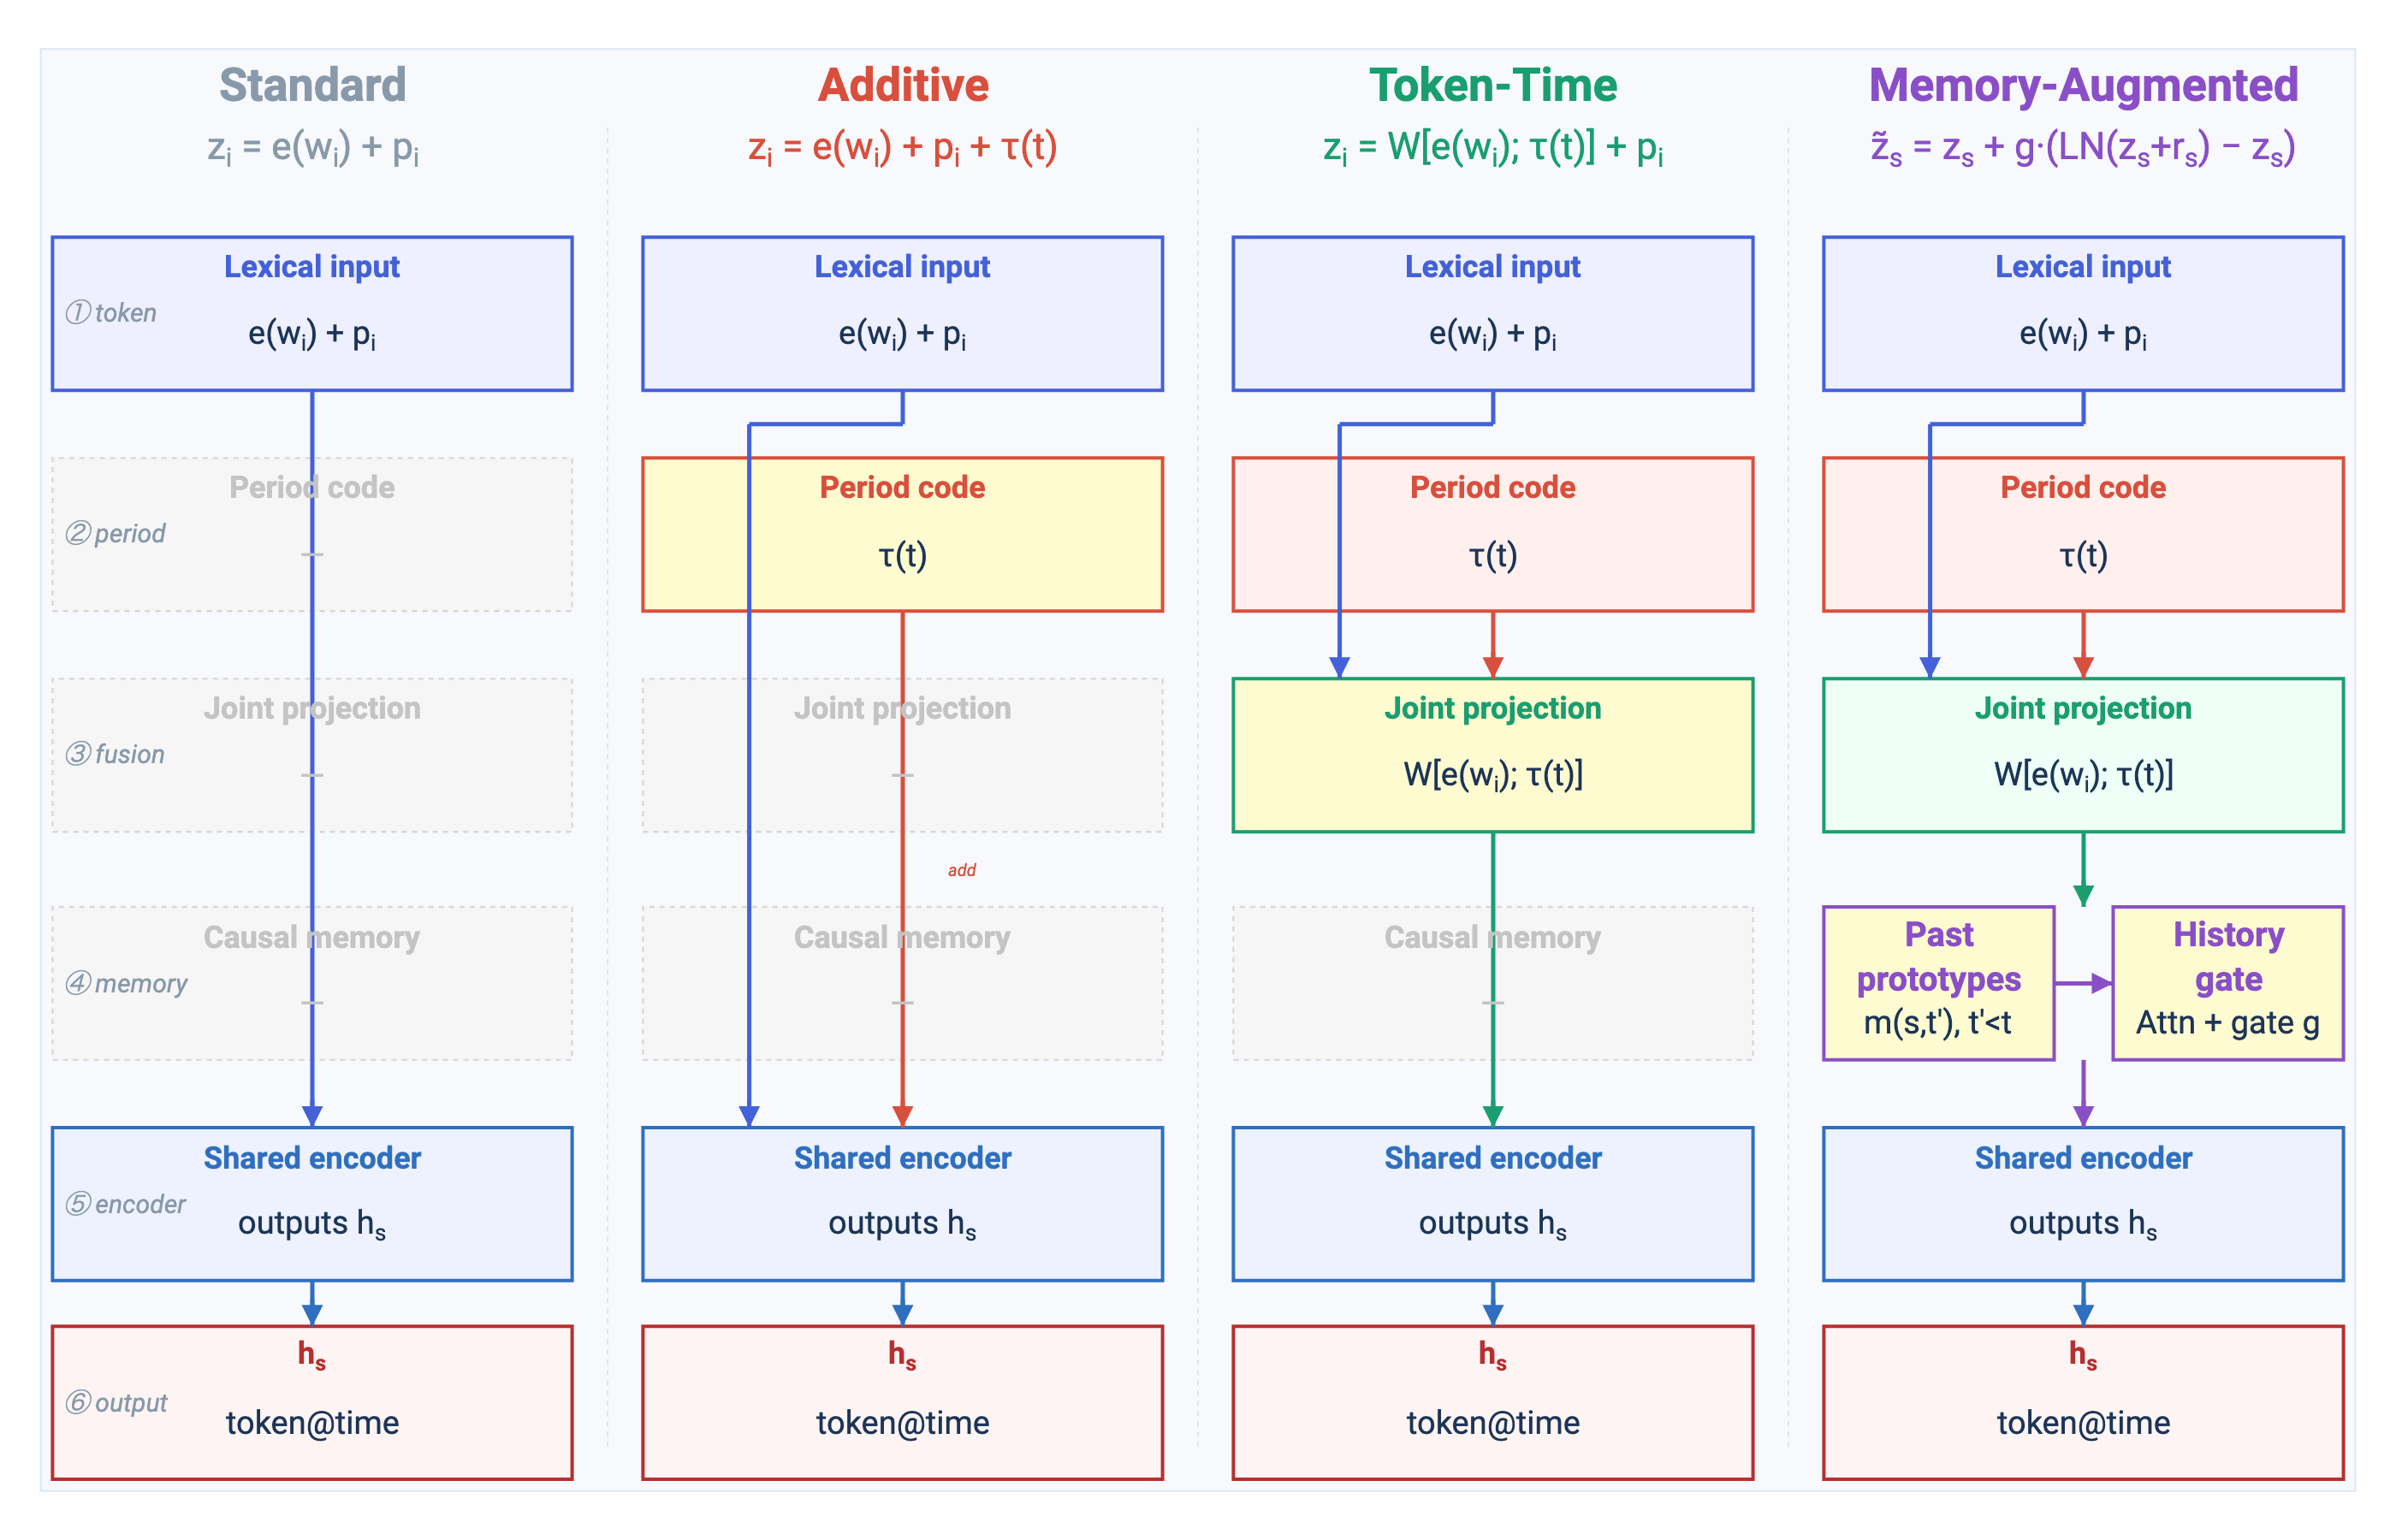
\includegraphics[width=\textwidth]{outputs/figures/figure2_architecture_detail.png}
\caption{Controlled design comparison. \textbf{Standard}: Transformer baseline
with no temporal signal. \textbf{Additive}: temporal baseline that adds the same
period vector to every token. \textbf{Token-Time}: Token-Time Transformer using joint
token-time projection. \textbf{Memory-Augmented}: extension of Token-Time with
Prototype Memory and Temporal Attention. New components are highlighted in
yellow; dashed grey boxes mark inactive
components.}
\label{fig:architecture}
\end{figure}

\subsection{Baseline: Standard Transformer}
Standard is the null hypothesis: no period signal is available, so any temporal
behavior must arise from changes in the observed words alone.
\[
  z_i = e(w_i) + p_i .
\]

\subsection{Baseline: Additive Time-Conditioned Transformer}
The Additive baseline tests whether a uniform global temporal signal suffices.
It adds the same period vector \(\tau(t)\) to every token:

\[
  z_i = e(w_i) + p_i + \tau(t).
\]

Now \texttt{S5 V2 O3} at \(t0\) and \(t9\) are distinguishable: the subject
receives \(\tau(0)\) or \(\tau(9)\). The same shift is applied to every token,
so Additive tells the whole sentence which period it belongs to but does not
bind period to individual token identities.

\subsection{Token-Time Transformer}
The Token-Time Transformer in Figure~\ref{fig:architecture}
asks whether exposing token identity and period jointly before self-attention is
enough. Instead of adding the same period vector to all tokens, Token-Time
concatenates each token embedding with \(\tau(t)\) and projects the pair:

\[
  z_i = W [e(w_i);\, \tau(t)] + p_i ,
\]

where \(e(w_i), \tau(t) \in \mathbb{R}^d\) and \(W \in \mathbb{R}^{d \times
2d}\). Although \(W\) is linear, it exposes token-period inputs before
self-attention and later nonlinear layers. Thus \texttt{S5} at \(t0\) and
\texttt{S5} at \(t9\) enter the encoder as distinct period-conditioned inputs.

\subsection{Memory-Augmented Extension}
The Memory-Augmented extension asks whether causal history helps beyond token-time
conditioning. It starts exactly like Token-Time: for a current sentence containing
\texttt{S5} at \(t7\), the model first builds token-time input embeddings for
\texttt{[CLS] S5 V O [SEP]}. It then modifies only the subject embedding before
the Transformer encoder sees the sentence.

The additional information comes from Prototype Memory. The extension stores one
prototype vector per subject and past period. A prototype \(m(s,t)\) is the
average representation of subject \(s\) across training sentences from period
\(t\). The memory is causal: at \(t7\), the model may consult
\(\{m(\texttt{S5},0),\ldots,m(\texttt{S5},6)\}\), but not prototypes from
\(t7\) or later.

Temporal attention turns this list of past prototypes into a history summary
for the current subject. Let \(z_s\) be the current Token-Time subject embedding and
let \(M_s\) be the matrix of available causal prototypes, one row per past
period. The attention operation uses \(z_s\) as the query and \(M_s\) as keys
and values:

\[
  r_s = \mathrm{Attn}(z_s, M_s, M_s).
\]

The vector \(r_s\) summarizes the parts of the subject's history that are most
relevant to the current period. A learned scalar gate \(g\) then decides how
much this history summary should change the current subject embedding:

\[
  \tilde{z}_s =
  z_s + g \cdot
  \left(\mathrm{LN}(z_s + r_s) - z_s\right).
\]

Here, \(\mathrm{LN}\) denotes layer normalization, and \(g\) is a learned
scalar gate initialized at zero so that the extension reduces to Token-Time at
initialization. Finally, \(\tilde{z}_s\) replaces \(z_s\) in the input
sequence; verb and object embeddings are unchanged, so the subject is the only
token that enters the encoder informed by causal prototype history.

\section{Evaluation Protocol and Diagnostics}
% Target length: 1.25--1.5 pages.
All models in the comparison chain are trained with masked language modeling
over the synthetic SVO corpus. The planted \texttt{true\_context} label is
withheld from training and used exclusively for post-hoc evaluation: it tests
whether the learned subject representation reflects the planted temporal
trajectory. The primary evaluation target is \(h_s\), the final hidden state
at the subject position, because subjects are the lexical items whose meanings
are designed to drift, remain stable, or bifurcate over time.

We use four diagnostics, each targeting a distinct aspect of temporal
representation.

\textbf{D1: Linear probe~\cite{conneau2018probing}.} Asks whether \(h_s\)
encodes the planted context label at all. The encoder is frozen; a linear
classifier is trained on \(h_s\) representations extracted from the held-out
test sentences of the standard (75\%-fidelity) split and evaluated on the
ambiguous and continuation splits. High accuracy indicates that
period-appropriate context is linearly separable in the representation, but
does not reveal whether that separation shifts systematically over time.

\textbf{D2: Context drift score.} Asks whether the neighborhood of a subject
shifts in the expected direction across periods. For each period and subject
class, we retrieve the \(k=10\) nearest neighbors of \(h_s\) by cosine
similarity (excluding the query itself) and record the proportion assigned to
$N_1$. A representation is traceable at period \(t\) if this proportion tracks
\(P(N_1 \mid s, t)\), the same probability that governs corpus generation at
that period. For drifting subjects, the proportion should therefore decrease
monotonically from $t0$ to $t9$; for stable subjects it should remain near its
initial value; for bifurcating subjects it should decrease less steeply, as the
representation splits between neighborhoods rather than migrating from one to
the other.

\textbf{D3: Contrastive diagnostic.} Asks whether the period label alone
drives representational change. We present the same sentence with two different
period labels and compute the sign-flip rate: the proportion of pairs for which
swapping the period reverses the nearest-neighbor assignment, from
$N_1$-dominant to $N_2$-dominant or vice versa. A model that ignores the period
input produces a sign-flip rate of zero; a model that responds to it produces a
rate above zero.

\textbf{D4: Continuation diagnostic.} Asks whether the learned temporal
mapping generalizes beyond training. We evaluate on held-out periods
\(t8\)--\(t9\), excluded from MLM training, and operationalize the diagnostic as
linear-probe accuracy on representations from these periods. A model that has
internalized the direction of change, rather than memorizing period-specific
patterns, should preserve context recoverability in unseen periods.

The four diagnostics are interpreted through a fixed comparison chain.
Additive vs.\ Standard isolates the effect of adding any temporal signal.
Token-Time vs.\ Additive tests whether joint token-time conditioning adds
anything beyond a uniform global signal; in this regime the effect is visible
only on the ambiguous-split probe. Memory-Augmented vs.\ Token-Time tests the
contribution of causal prototype memory, the mechanism most expected to affect
D3 and D4.

For the Memory-Augmented extension, we include an \textit{oracle-memory}
diagnostic: learned prototypes are replaced by fixed vectors encoding the true
historical \(P(N_1 \mid s,t)\) trajectory, with the rest of the architecture
unchanged. This isolates whether the failure of learned prototypes is due to the
memory pathway itself or to the aggregation mechanism; improvement under oracle
prototypes indicates that the pathway can use better historical signals, while
learned mean prototypes remain the weak point.

\section{Results}
% Target length: 2.5--3.0 pages.
We report means and 95\% confidence intervals over 31 training seeds.
Conditioning of any form substantially moves drifting subjects relative to the
non-temporal baseline: all three conditioned models reach \(\Delta\approx-0.56\)
vs.\ \(-0.221\) for Standard, more than doubling the neighborhood displacement.
Additive and Token-Time are indistinguishable on aggregate drift in this
controlled setting. Memory-Augmented does not improve over Token-Time.

\paragraph{Implementation details.}
All models share the same Transformer encoder: \(d=64\), 4 attention heads, 2
layers, feed-forward width 128, dropout 0.1. The period encoding projects 32
sinusoidal features of \(t/T\) to \(d\) via a two-layer MLP. Training uses
AdamW (lr \(=10^{-3}\), weight decay \(=10^{-2}\)) with a cosine annealing
schedule, 30 epochs, batch size 64. The corpus contains 5{,}000 SVO sentences;
MLM training uses 3{,}159 sentences from periods \(t0\)--\(t7\); 763 sentences
from the same periods form the held-out evaluation set; 794 sentences from
\(t8\)--\(t9\) are reserved for the continuation diagnostic.

\subsection{Temporal Neighborhood Movement}
% Main claim: temporal conditioning produces stronger neighborhood transitions than Standard.
% Use class-specific curves to avoid claiming stable subjects are perfectly flat.
Figure~\ref{fig:context-drift} and Table~\ref{tab:context-drift} show the
context drift score across periods. Standard reaches \(\Delta=-0.221\)
(95\% CI \([-0.240, -0.203]\)); Token-Time reaches \(\Delta=-0.563\), more
than doubling the displacement. Additive reaches an equivalent value
(\(\Delta=-0.567\)), confirming that a global temporal signal reproduces
aggregate drift in this high-fidelity setting.

The class-specific curves serve as controls (Table~\ref{tab:context-drift}).
Stable subjects show smaller movement in absolute magnitude (\(\Delta\) between
\(-0.150\) and \(-0.180\) for conditioned models, versus \(\Delta \approx -0.56\)
for drifting subjects), but the direction is consistently negative. This reflects
a global displacement of the embedding space induced by the period vector: even
subjects with flat planted trajectories are pulled along the learned temporal
direction, at lower magnitude. Bifurcating subjects show
intermediate drift: conditioned models reach \(t9\) values near \(0.53\),
matching the planted endpoint \(P(N_1 \mid s, t9) \approx 0.5\) for the
mixed state. The geometric diagnostic distinguishes all
three trajectory classes without relying on probe accuracy alone.

Paired equivalence testing (TOST, \(\delta=0.05\)) formalizes this:
diff\(=-0.003\), 90\% CI \([-0.026,\,+0.019]\), \(p_\mathrm{TOST}<0.001\);
equivalence holds also at \(\delta=0.034\) (\(p_\mathrm{TOST}=0.014\)). D2 thus confirms the geometric effect of joint conditioning; it is not a
comparison between conditioning strategies.

\begin{figure}[t]
\centering
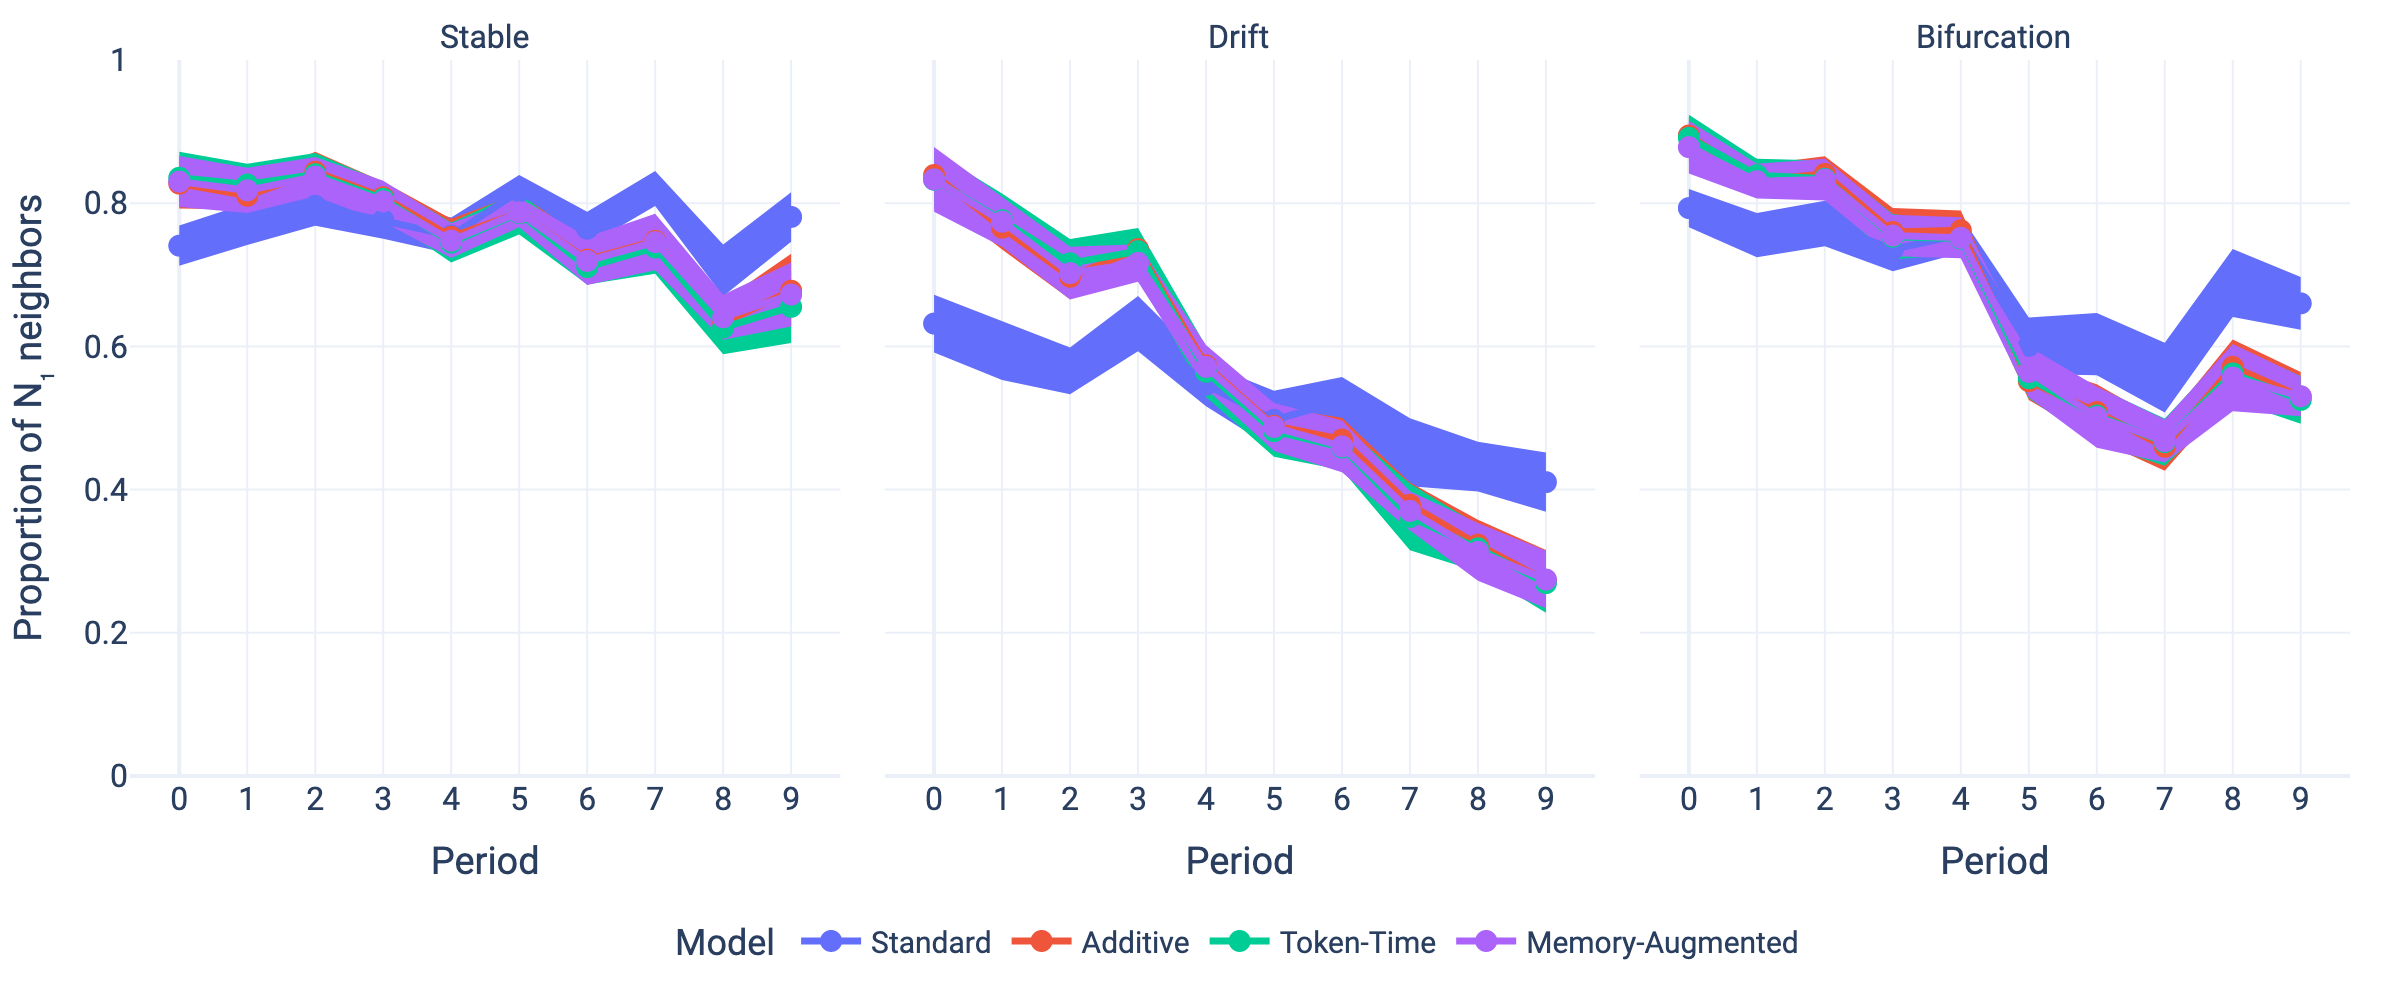
\includegraphics[width=\textwidth]{outputs/figures/figure3_context_drift.png}
\caption{Context drift score across periods. All conditioned models move drifting
subjects from $N_1$ toward $N_2$ more than Standard; Additive, Token-Time, and
Memory-Augmented produce similar trajectories. Stable and bifurcating subjects
provide class-specific controls.}
\label{fig:context-drift}
\end{figure}

\begin{table}[t]
\caption{Context drift score at the first and last periods. Values are means
over 31 seeds; \(\Delta=t9-t0\); 95\% CI half-widths in brackets.}
\label{tab:context-drift}
\centering
\scriptsize
\renewcommand{\arraystretch}{0.88}
\setlength{\tabcolsep}{4pt}
\begin{tabular}{llccc}
\toprule
\textbf{Class} & \textbf{Model} & \textbf{t0} & \textbf{t9} & \(\boldsymbol{\Delta}\) [CI\(_{\pm}\)] \\
\midrule
Stable & Standard & 0.741 & 0.781 & $+$0.040 [$\pm$0.017] \\
       & Additive & 0.827 & 0.678 & $-$0.150 [$\pm$0.027] \\
       & Token-Time    & 0.835 & 0.655 & $-$0.180 [$\pm$0.024] \\
       & Mem-Aug. & 0.830 & 0.672 & $-$0.158 [$\pm$0.021] \\
\midrule
Drift  & Standard & 0.632 & 0.410 & $-$0.221 [$\pm$0.018] \\
       & Additive & 0.839 & 0.272 & $-$0.567 [$\pm$0.019] \\
       & Token-Time    & 0.833 & 0.269 & $-$0.563 [$\pm$0.020] \\
       & Mem-Aug. & 0.833 & 0.274 & $-$0.559 [$\pm$0.022] \\
\midrule
Bifurc. & Standard & 0.793 & 0.660 & $-$0.133 [$\pm$0.018] \\
        & Additive & 0.895 & 0.530 & $-$0.365 [$\pm$0.017] \\
        & Token-Time    & 0.891 & 0.525 & $-$0.366 [$\pm$0.016] \\
        & Mem-Aug. & 0.878 & 0.530 & $-$0.348 [$\pm$0.015] \\
\bottomrule
\end{tabular}
\end{table}

\subsection{Probe and Contrastive Diagnostics}
The linear probe results reveal a distinction that drift score does not.
On the standard (75\%-fidelity) split, where local markers carry reliable
context signal, all conditioned models outperform Standard
(\(0.875\) [\(\pm\)0.005]): Additive reaches \(0.892\) [\(\pm\)0.003],
Token-Time \(0.881\) [\(\pm\)0.005], and Mem-Aug.\ \(0.881\) [\(\pm\)0.006];
on this split Additive is above Token-Time. The ordering reverses on the
ambiguous split, where local verb and object markers are uninformative: Standard
reaches \(0.565\) \([0.561, 0.568]\), Additive \(0.579\) \([0.575, 0.584]\),
Token-Time \(0.595\) \([0.589, 0.601]\), and Memory-Augmented \(0.598\)
\([0.590, 0.606]\). The confidence intervals for Additive and Token-Time do not
overlap, showing a reproducible advantage for joint token-time conditioning when
only subject identity and period remain as evidence. On the continuation split,
Additive and Token-Time reach the same accuracy (\(0.763\); Table~\ref{tab:main-results}),
matching their overlap on drift score. Probe accuracy alone is insufficient to establish temporal traceability because
it measures recoverability of the planted label, not neighborhood geometry.
Even so, the split-dependent ordering is preliminary evidence that the D2
equivalence is regime-specific: joint conditioning encodes temporal information
more precisely when local markers are removed.

The contrastive sign-flip rates are similar across conditioned models: Standard
\(0.000\), Additive \(0.602\) \([0.549, 0.655]\), Token-Time \(0.624\)
\([0.576, 0.673]\), Mem-Aug.\ \(0.587\) \([0.536, 0.638]\). Confidence
intervals overlap, so the contrastive diagnostic does not separate the
conditioned models.
\begin{table}[t]
\caption{Main traceability diagnostics (means, 31 seeds). Drift: context drift
score \(\Delta\) for drifting subjects; Flip: contrastive sign-flip rate (D3);
Ambig./Cont.: linear-probe accuracy on \(h_s\). 95\% CI in brackets.}
\label{tab:main-results}
\centering
\scriptsize
\renewcommand{\arraystretch}{0.88}
\setlength{\tabcolsep}{4pt}
\begin{tabular}{lcccc}
\toprule
\textbf{Model} & \textbf{Drift} & \textbf{Flip} & \textbf{Ambig.} & \textbf{Cont.} \\
\midrule
Standard & $-$0.221 [$\pm$0.018] & 0.000 & 0.565 [$\pm$0.004] & 0.730 [$\pm$0.004] \\
Additive & $-$0.567 [$\pm$0.019] & 0.602 [$\pm$0.053] & 0.579 [$\pm$0.005] & 0.763 [$\pm$0.003] \\
Token-Time    & $-$0.563 [$\pm$0.020] & 0.624 [$\pm$0.048] & 0.595 [$\pm$0.006] & 0.763 [$\pm$0.004] \\
Mem-Aug. & $-$0.559 [$\pm$0.022] & 0.587 [$\pm$0.051] & 0.598 [$\pm$0.008] & 0.755 [$\pm$0.005] \\
\bottomrule
\end{tabular}
\end{table}

\subsection{Memory Diagnostics}
% Memory-Augmented: not a stable improvement over Token-Time; oracle diagnostic
% localizes the limitation to mean-prototype aggregation.
The Memory-Augmented extension does not improve over Token-Time. Across 31
seeds, learned prototypes reach a continuation
accuracy of \(0.755\) \([0.750, 0.760]\), marginally below Token-Time at
\(0.763\) \([0.759, 0.766]\) (\(\Delta=-0.008\)). The oracle diagnostic
shows the limits of this architecture: replacing learned prototypes with fixed
vectors encoding the true \(P(N_1 \mid s, t)\) trajectory yields a
continuation of \(0.769\) \([0.761, 0.777]\) and a sign-flip rate of \(0.694\)
\([0.576, 0.812]\), versus \(0.624\) for Token-Time. The sign-flip difference
(\(\Delta=+0.070\)) exceeds the continuation improvement
(\(\Delta=+0.007\)), but both CIs are wide. The MLM objective optimizes token
prediction, not trajectory geometry. Perfect historical prototypes can improve
contrastive behavior, which depends on local period sensitivity, but they do not
replace a training signal for geometric continuity across unseen periods.

\begin{table}[t]
\caption{Memory diagnostics (means, 31 seeds). Continuation (D4): linear-probe
accuracy on held-out periods \(t8\)--\(t9\); Flip: contrastive sign-flip rate
(D3); 95\% CI half-widths in brackets.}
\label{tab:memory-diagnostics}
\centering
\scriptsize
\renewcommand{\arraystretch}{0.88}
\setlength{\tabcolsep}{4pt}
\begin{tabular}{lccc}
\toprule
\textbf{Model} & \textbf{Cont.} & \textbf{Flip} & \textbf{$\Delta$ cont.\ vs.\ Token-Time} \\
\midrule
Token-Time (ref.)  & 0.763 [$\pm$0.004] & 0.624 [$\pm$0.048] & -- \\
Mem-Aug.\ learned  & 0.755 [$\pm$0.005] & 0.587 [$\pm$0.051] & $-$0.008 [$\pm$0.006] \\
Mem-Aug.\ oracle   & 0.769 [$\pm$0.004] & 0.694 [$\pm$0.059] & $+$0.007 [$\pm$0.007] \\
\bottomrule
\end{tabular}
\end{table}

\section{Discussion and Conclusion}
% Target length: 1.25--1.5 pages.
Conditioned models improve neighborhood drift substantially
(\(\Delta\approx-0.563\) vs.\ \(-0.221\) for Standard), but no architecture
matches the planted trajectories across all diagnostics: even oracle memory
raises continuation accuracy only to \(0.769\). The pattern points to the MLM
objective, which rewards token prediction rather than geometric consistency
across periods; traceability appears only as a by-product.

In this controlled, high-fidelity setting Additive and Token-Time are equivalent
on aggregate drift score (TOST, \(\delta=0.05\), \(p_\mathrm{TOST}<0.001\)):
a global temporal signal suffices to reproduce neighborhood movement under
reliable local markers, and adjudication between conditioning strategies across
noise regimes is left for future work. The only reproducible distinction appears
on the ambiguous split (\(0.595\) vs.\ \(0.579\), non-overlapping CIs), where
local markers carry no signal: preliminary evidence that joint conditioning
encodes temporal information more precisely in harder conditions. Layer-wise CKA corroborates this: Additive vs.\ Token-Time similarity increases
from 0.726 to 0.887 across encoder depth (Standard stays near 0.22), suggesting
self-attention absorbs the input-level difference.

The Memory-Augmented extension points to a second failure mode. For
bifurcating subjects, which develop two coexisting senses in later periods, a
mean prototype lies between clusters and represents neither well. The oracle
diagnostic shows that the memory pathway can use better historical signals:
fixed vectors encoding the true \(P(N_1 \mid s, t)\) trajectory increase the
sign-flip rate by \(+0.070\) over Token-Time (\(0.694\) vs.\ \(0.624\)). The
learned mean prototypes cannot preserve the internal structure of a word's
sense distribution; geometry-based mode-separation metrics confirm no
architecture outperforms Additive in separating the two sense clusters for
bifurcating subjects.

These conclusions come from controlled diagnostics, not open-domain diachronic
language. The probe-level advantage of Token-Time over Additive is statistically
stable but modest (1.6 percentage points) and does not appear on the drift
score; it may not generalize beyond fixed subject positions and a small
vocabulary. The suite was co-designed with the evaluated architectures to characterize them;
the paper does not claim it as an independent validation of any architecture as
a definitive solution to temporal traceability.

Two directions remain open. First, Token-Time layer-0 heads show greater
temporal variance in attention mass (L0H3: 0.0075 vs.\ Additive 0.0033), yet
ablating individual heads only partially reduces representational alignment
(L0H0: \(\Delta=-0.026\); L0H1: \(\Delta=-0.021\)), suggesting a distributed
effect; a pilot noise sweep (3 seeds, slope\(=+1.07\), \(p=0.002\)) is
consistent with Token-Time retaining a drift advantage under degraded markers,
but needs replication across noise regimes and natural corpora. Second, memory
mechanisms need to preserve the internal structure of historical representations
rather than collapsing each period to a single prototype, the primary open
problem for bifurcating subjects.

% Bibliography
\bibliographystyle{splncs04}
\bibliography{references}

\end{document}
